%******************************************************************************%
% Copyright (C) 2018  Louis Solofrizzo                                         %
%                                                                              %
% This content is considered a free software: you can redistribute it          %
% and/or modify it under the terms of the GNU General Public License as        %
% published by the Free Software Foundation, either version 3 of the License,  %
% or (at your option) any later version.                                       %
%                                                                              %
% This program is distributed in the hope that it will be useful,              %
% but WITHOUT ANY WARRANTY; without even the implied warranty of               %
% MERCHANTABILITY or FITNESS FOR A PARTICULAR PURPOSE.  See the                %
% GNU General Public License for more details.                                 %
%                                                                              %
% You should have received a copy of the GNU General Public License            %
% along with this program.  If not, see <https://www.gnu.org/licenses/>.       %
%******************************************************************************%

%******************************************************************************%
%                                                                              %
%                          KFS_6.en.tex for KFS_6                              %
%                                                                              %
%                  Created on : Wed May 25 13:27:28 2016                       %
%          Made by : Louis "Ne02ptzero" Solofrizzo <louis@ne02ptzero.me>       %
%                                                                              %
%******************************************************************************%

\documentclass{42-en}


%******************************************************************************%
%                                                                              %
%                                    Header                                    %
%                                                                              %
%******************************************************************************%
\begin{document}



                           \title{KFS\_6}
                          \subtitle{Filesystem}
                       \member{Louis Solofrizzo}{louis@ne02ptzero.me}
                        \member{42 Staff}{pedago@42.fr}

\summary {
    Disk, files and format!
}

\maketitle

\tableofcontents


%******************************************************************************%
%                                                                              %
%                                  Foreword                                    %
%                                                                              %
%******************************************************************************%
\chapter{Foreword}
    I don't have any idea for this foreword. So here's a penguin:\\
    \centerline{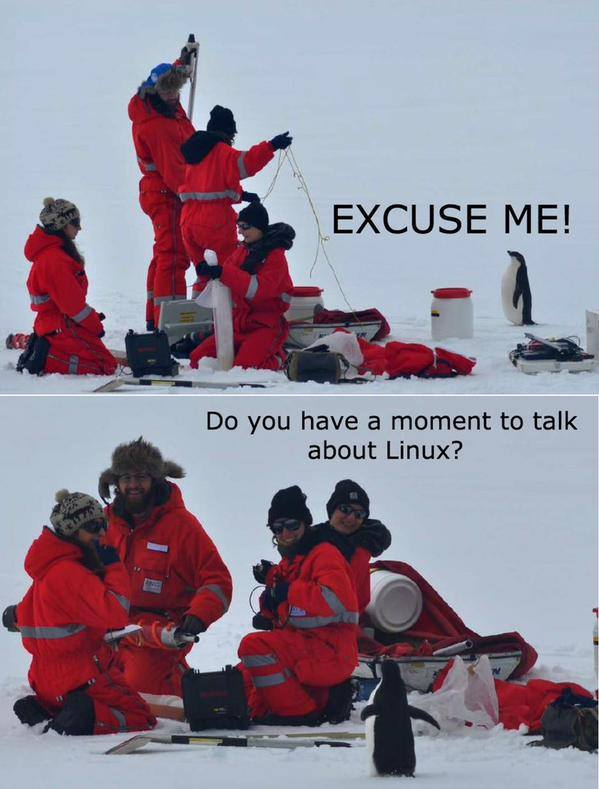
\includegraphics[width=12cm]{oui.jpg}}
    A good one.

%******************************************************************************%
%                                                                              %
%                                 Introduction                                 %
%                                                                              %
%******************************************************************************%
\chapter{Introduction}
    Filesystem! Finally, some files in our kernel.
    We have two things to discuss:
    \subsection{Filesystem}
    Let's see the wikipedia definition, but I'm sure you all know what a
    filesystem is by now:
    \begin{quotation}
        \textit{In computing, a file system (or filesystem) is used to control 
        how data is stored and retrieved. Without a file system, information 
        placed in a storage area would be one large body of data with no way to 
        tell where one piece of information stops and the next begins. By 
        separating the data into pieces and giving each piece a name, the 
        information is easily isolated and identified. Taking its name from 
        the way paper-based information systems are named, each group of data 
        is called a "file". The structure and logic rules used to manage the 
        groups of information and their names is called a "file system".}
    \end{quotation}
    Nothing to add here, I'm sure you're all comfortable with the concept of
    files.
    \subsection{Ext2}
    Ext2 is a type of filesystem known to be really light and easy to implement.
    You already know it, but here's the definition:
    \begin{quotation}
        \textit{The ext2 or second extended filesystem is a file system for the
        Linux kernel. It was initially designed by Rémy Card as a replacement
        for the extended file system (ext). Having been designed according to
        the same principles as the Berkeley Fast File System from BSD, it was
        the first commercial-grade filesystem for Linux.
        The canonical implementation of ext2 is the "ext2fs" filesystem driver
        in the Linux kernel. Other implementations (of varying quality and
        completeness) exist in GNU Hurd, MINIX 3, some BSD kernels, in MiNT,
        and as third-party Microsoft Windows and OS X drivers.
        ext2 was the default filesystem in several Linux distributions,
        including Debian and Red Hat Linux, until supplanted more recently by
        ext3, which is almost completely compatible with ext2 and is a
        journaling file system. ext2 is still the filesystem of choice for
        flash-based storage media (such as SD cards, and USB flash drives),
        since its lack of a journal increases performance and minimizes the
        number of writes, and flash devices have a limited number of write
        cycles. However, recent Linux kernels support a journal-less mode of
        ext4 which provides benefits not found with ext2.}
        \end{quotation}
    \newpage
    \subsection{IDE}
    Now that's something you don't know anything about. Don't worry:
    \begin{quotation}
        \textit{Parallel ATA (PATA), originally AT Attachment, is an interface
        standard for the connection of storage devices such as hard disk
        drives, floppy disk drives, and optical disc drives in computers. The
        standard is maintained by the X3/INCITS committee. It uses the
        underlying AT Attachment (ATA) and AT Attachment Packet Interface
        (ATAPI) standards.
        The Parallel ATA standard is the result of a long history of
        incremental technical development, which began with the original AT
        Attachment interface, developed for use in early PC AT equipment. The
        ATA interface itself evolved in several stages from Western Digital's
        original Integrated Drive Electronics (IDE) interface. As a result,
        many near-synonyms for ATA/ATAPI and its previous incarnations are
        still in common informal use, in particular Extended IDE (EIDE) and
        Ultra ATA (UATA). After the introduction of Serial ATA (SATA) in 2003,
        the original ATA was renamed to Parallel ATA, or PATA for short.
        The term Integrated Drive Electronics refers not just to the connector
        and interface definition, but also to the fact that the drive
        controller is integrated into the drive, as opposed to a separate
        controller on or connected to the motherboard. The interface cards used
        to connect a parallel ATA drive to, for example, a PCI slot are not
        drive controllers: they are merely bridges between the host bus and the
        ATA interface. Since the original ATA interface is essentially just a
        16-bit ISA bus in disguise, the bridge was especially simple in case of
        an ATA connector being located on an ISA interface card. The integrated
        controller presented the drive to the host computer as an array of
        512-byte blocks with a relatively simple command interface. This
        relieved the mainboard and interface cards in the host computer of the
        chores of stepping the disk head arm, moving the head arm in and out,
        and so on, as had to be done with earlier ST-506 and ESDI hard drives.
        All of these low-level details of the mechanical operation of the drive
        were now handled by the controller on the drive itself. This also
        eliminated the need to design a single controller that could handle
        many different types of drives, since the controller could be unique
        for the drive. The host need only ask for a particular sector, or
        block, to be read or written, and either accept the data from the drive
        or send the data to it.}
    \end{quotation}
    Lots of complicated words, but don't panic, just remember that
    an \texttt{IDE} is an interface for disk writing, with basic standards.
    It's one of the simplest interfaces out there, easy to implement.
    Let's talk about it in more detail.
    \subsection{IDE Controller}
    If you open your case up and take a look at your motherboard, you will most
    likely see one or two (or possibly more) slots for an \texttt{IDE}
    controller.\\
    The white and green ports are IDE ports, also known as
    channels. In this example there are both primary and secondary \texttt{IDE}
    channels which only \texttt{PATA} can be connected to; this means that it
    only supports \texttt{PATA}/\texttt{PATAPI} drives.\\
    Each port can have a \texttt{PATA} cable connected to it. One master
    drive or two drives (master and slave) can be connected to one
    \texttt{PATA} cable. So that leaves us with the following possibilities:
    \begin{itemize}\itemsep1pt
        \item Primary Master Drive.
        \item Primary Slave Drive.
        \item Secondary Master Drive.
        \item Secondary Slave Drive.
    \end{itemize}
    Each drive can be either \texttt{PATA} or \texttt{PATAPI}.  Each
    \texttt{IDE} controller appears as a device on the \texttt{PCI} bus. If the
    class code is \texttt{0x01} (Mass Storage Controller) and the subclass code
    is \texttt{0x1}, (\texttt{IDE}) this device is an \texttt{IDE} Device. The
    \texttt{IDE} device only uses five BARs out of the six ones.
    \begin{itemize}\itemsep1pt
    \item \texttt{BAR0}: Base address of primary channel (I/O space),
        if it is \texttt{0x0} or \texttt{0x1}, the port is \texttt{0x1F0}.
    \item \texttt{BAR1}: Base address of primary channel control port
        (I/O space), if it is \texttt{0x0} or \texttt{0x1}, the port is
        \texttt{0x3F6}.
    \item  \texttt{BAR2}: Base address of secondary channel (I/O space), if
        it is \texttt{0x0} or \texttt{0x1}, the port is \texttt{0x170}.
    \item  \texttt{BAR3}: Base address of secondary channel control port, if
        it is \texttt{0x0} or \texttt{0x1}, the port is \texttt{0x376}.
    \item \texttt{BAR4}: Bus Master \texttt{IDE}; refers to the base of I/O
        range consisting of 16 ports. All 8 ports control DMA on the primary
        and secondary channel respectively.
    \end{itemize}



%******************************************************************************%
%                                                                              %
%                                  Goals                                       %
%                                                                              %
%******************************************************************************%
\chapter{Goals}

    At the end of this project, you will add the following to your kernel:
    \begin{itemize}\itemsep1pt
        \item A complete interface to read / write an \texttt{IDE}.
        \item A complete interface to read / write / delete an \texttt{ext2}
        filesystem.
        \item A basic file tree (/sys, /var, /dev, /proc, /sys).
    \end{itemize}


%******************************************************************************%
%                                                                              %
%                             General instructions                             %
%                                                                              %
%******************************************************************************%
\chapter{General instructions}
    \section{Code and Execution}
        \subsection{Emulation}
        The following part is not mandatory, you're free to use any virtual
        manager you want; however, I suggest you use \texttt{KVM}.
        It's a \texttt{Kernel Virtual Manager} with advanced execution
        and debug functions.
        All of the examples below will use \texttt{KVM}.
        \subsection{Language}
            The \texttt{C} language is not mandatory, you can use any language
            you want for this series of projects.\\
            Keep in mind that not all languages are kernel friendly, you could
            code a kernel in \texttt{Javascript}, but are you sure it's a
            good idea?\\
            Also, most of the documentation is written in \texttt{C}, you will
            have to 'translate' the code all along if you choose a different
            language.\\

            Furthermore, not all the features of a given language can be used
            in a basic kernel. Let's take an example with \texttt{C++}:\\
            this language uses 'new' to make allocations, classes and
            structures declarations. But in your kernel you don't have a memory
            interface (yet), so you can't use any of these features.\\

            Many languages can be used instead of \texttt{C},
            like \texttt{C++}, \texttt{Rust}, \texttt{Go}, etc.
            You can even code your entire kernel in \texttt{ASM}!\\
            \begin{center}
              
\includegraphics[width=8cm]{choose.jpg}
            \end{center}

\newpage


    \section{Compilation}
        \subsection{Compilers}
            You can choose any compiler you want. I personaly use \texttt{gcc}
            and \texttt{nasm}. A Makefile must be turned-in as well.
        \subsection{Flags}
            In order to boot your kernel without any dependency, you must
            compile your code with the following flags (adapt the flags for
            your language, these are \texttt{C++} examples):
            \begin{itemize}\itemsep1pt
                \item \texttt{-fno-builtin}
                \item \texttt{-fno-exception}
                \item \texttt{-fno-stack-protector}
                \item \texttt{-fno-rtti}
                \item \texttt{-nostdlib}
                \item \texttt{-nodefaultlibs}
            \end{itemize}
            You might have noticed these two flags: \texttt{-nodefaultlibs}
            and \texttt{-nostdlib}. Your Kernel will be compiled on a host
            system, that's true, but it cannot be linked to any existing
            library on that host, otherwise it will not be executed.
    \section{Linking}
        You cannot use an existing linker in order to link your kernel.
        As mentionned above, your kernel would not be initialized. So you must
        create a linker for your kernel.\\
        Be carefull, you \texttt{CAN} use the 'ld' binary available on your
        host, but you \texttt{CANNOT} use the .ld file of your host.
    \section{Architecture}
        The \texttt{i386} (x86) architecture is mandatory (you can thank
        me later).
    \section{Documentation}
        There is a lot of documentation available, good and bad.
        I personaly think the \texttt{\href{http://wiki.osdev.org/Main_Page}
        {OSDev}} wiki is one of the best.
    \section{Base code}
        In this subject, you have to take your previous \texttt{KFS} code,
        and work from it!\\
        Or don't. And rewrite everything from scratch. Your call!
\newpage

%******************************************************************************%
%                                                                              %
%                             Mandatory part                                   %
%                                                                              %
%******************************************************************************%
\chapter{Mandatory part}

    For this subject, you will have to implement a complete and functional
    filesystem interface. Let's see that, point by point:
    \begin{itemize}\itemsep1pt
        \item Write a complete interface to read / write an IDE.
        \item Write a complete interface to read an ext2 filesystem:
        \begin{itemize}\itemsep1pt
            \item Read the ext2 headers.
            \item Create and fill in an ext2 kernel-side structure with groups,
            super blocks, blocks and inodes.
        \end{itemize}
        \item Write a complete structure for a filesystem. That includes:
        \begin{itemize}\itemsep1pt
            \item Name
            \item Size
            \item Type
            \item Inode
            \item Links
            \item Master
            \item Father
            \item Children
            \item Rights
            \item Next of kin
        \end{itemize}
    \end{itemize}
    You will have to implement a \texttt{cat} command in your console, with
    the behavior of the original \texttt{cat}. Now that you have a root
    directory, you need to code a directory change too (pwd / cd) in your
    console. Keep in mind that a process needs to have its own pwd, and two
    processes can have different pwds at the same time.


%******************************************************************************%
%                                                                              %
%                                 Bonus part                                   %
%                                                                              %
%******************************************************************************%
\chapter{Bonus part}

    For the bonuses, you will have to handle multiple partitions, mount and
    demount.\\
    You can, also, implement users (with passwords, logins, etc.).


%******************************************************************************%
%                                                                              %
%                           Turn-in and peer-evaluation                        %
%                                                                              %
%******************************************************************************%
\chapter{Turn-in and peer-evaluation}
    Turn your work in using your \texttt{GiT} repository, as
    usual. Only the work present on your repository will be graded in the
    evaluation.

    Your must turn in your code, a Makefile and a basic virtual image for your
    kernel.\\
    Side note about that image, THERE IS NO NEED TO BE BUILT LIKE AN ELEPHANT.


%******************************************************************************%
\end{document}
